\documentclass[zh]{resume}
\usetikzlibrary{calc}
\iconsize{\Large}

\name{妍}{汪}

\profile{
  \birthday{1999}
  \mobile{19905183012}
  \email{793701633@qq.com}
}

% 调整全局字体大小
\renewcommand{\normalsize}{\fontsize{11pt}{13.2pt}\selectfont}

\begin{document}

% 右上角添加头像
\begin{tikzpicture}[remember picture, overlay]
  \node[anchor = north east] at ($(current page.north east)+(-2cm, -0.5cm)$) {
    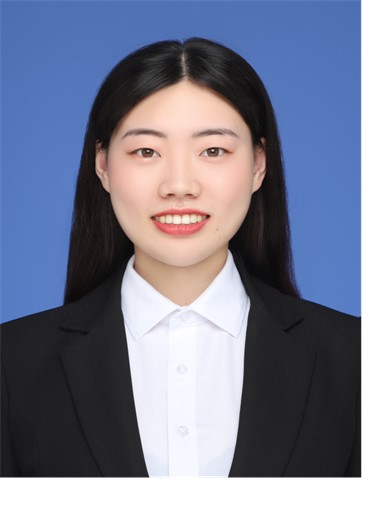
\includegraphics[height=3.5cm]{汪妍简历头像.jpg}
  };
\end{tikzpicture}

\makeheader

% ==========================================================
% 1. 教育背景
% ==========================================================
\sectionTitle{教育背景}{\degreeSymbol}
\begin{itemize}
  \setlength{\itemsep}{3pt} \setlength{\parsep}{0pt}
  \item \textbf{南京医科大学康达学院} \hfill 护理学 \hfill \textbf{学士} (2019.09 -- 2021.07) \\
  获学院优秀学生奖学金（三等）、优秀实习生
  \item \textbf{江苏护理职业学院} \hfill 助产专业 \hfill \textbf{专科} (2014.09 -- 2019.07) \\
  国家励志奖学金、学院一等奖学金（多次）、三好学生、优秀毕业生
\end{itemize}

% ==========================================================
% 2. 工作经历
% ==========================================================
\sectionTitle{工作经历}{\homeSymbol}
\begin{itemize}
    \item \textbf{南京大学医学院附属鼓楼医院 | 泌尿外科 | 护师} \hfill \textbf{2021.07 -- 至今}
    \begin{itemize}
        \item 负责泌尿外科围术期患者护理，熟练掌握前列腺增生微创术后患者管理
        \item 独立完成经尿道前列腺热蒸汽消融术（Rezum）患者术前评估、术后观察及康复指导
        \item 参与科室护理质量改进，承担患者健康教育和心理护理工作
        \item 具有院内多科室轮转经验，积累了扎实的临床护理基础
        \item 作为积极分子积极参与院内抗疫工作，展现良好的职业素养和奉献精神
        \item 工作态度积极，服务质量优异，收到患者及家属表扬信20余封、锦旗1面
    \end{itemize}
\end{itemize}

% ==========================================================
% 3. 科研经历
% ==========================================================
\sectionTitle{科研经历}{\infoSymbol}

\begin{itemize}
        \item
        \textbf{第一作者论文（投稿中）} \hfill \textbf{2024.01 -- 至今}
          \\
        \textbf{论文题目: } 《基于时效性激励理论的护理干预在经尿道前列腺热蒸汽消融术患者的应用效果研究》
        \\
        \textbf{研究内容: } 采用随机对照试验（RCT）设计，纳入100例BPH手术患者，观察组实施基于时效性激励理论（情感激励、需要激励、榜样激励、利益激励）的系统化护理干预。结果显示：干预组IPSS评分、SAS/SDS评分及VAS评分均显著低于对照组（\textbf{P<0.001}），控尿能力、治疗依从性和满意度显著提升（\textbf{P<0.05}）。独立完成研究方案设计、数据采集分析（SPSS 22.0）及论文撰写。

        \item
        \textbf{参与科研项目} \hfill \textbf{2024 -- 2025}
        \begin{itemize}
            \item 南京鼓楼医院/南京大学中国医院改革发展研究院项目（NDYGN2024085）
            \item 南京鼓楼医院护理科研项目（2025-H477）
        \end{itemize}
\end{itemize}

% ==========================================================
% 4. 奖项与证书
% ==========================================================
\sectionTitle{奖项与证书}{\birthdaySymbol}

\twocolumnsection{
\begin{itemize}
    \item \textbf{学校期间（2014-2021）}
    \item 5.12护士节婴儿抚触技能竞赛三等奖（2017）
    \item 国家励志奖学金（2018）
    \item 学院一等奖学金（多次）
    \item 学院精业之星（学习标兵）
    \item 三好学生、优秀毕业生
\end{itemize}
}{
\begin{itemize}
    \item \textbf{工作期间（2021至今）}
    \item 第二届心理微视频竞赛三等奖、最佳人气奖（2024）
    \item \textbf{证书}
    \item 护士执业资格证书
    \item 大学英语四级（CET-4）
    \item 医护英语水平考试二级、三级
    \item 全国计算机一级合格
    \item 普通话二级甲等
\end{itemize}
}

\end{document}
